\chapter{Stereo vision system operational concept}

This chapter defines the operational concept of the LINKU stereo vision system and its role within the mission architecture. The system is intended to provide direct visual information about the deployment state, spatial geometry, and dynamic behavior of the tethered satellite configuration throughout the mission.
\\\\
Unlike conventional telemetry sensors, which provide localized or indirect measurements, the stereo vision system is designed to extract geometric information about the tether's physical shape and spatial evolution. This capability is particularly relevant during deployment and post-deployment operations, where the tether may experience oscillations, curvature, transient instabilities, or partial out-of-plane motion.
\\\\
The stereo vision system is therefore conceived as a complementary observation instrument that supports both operational monitoring and post-processing geometric analysis. Its functionality is closely linked with other onboard measurements, including GNSS data, inertial sensing, and tether-tension measurements, which together provide a more complete characterization of the tethered system dynamics.

\section{Mission operational stages and observational objectives}

The stereo vision system operates during two principal operational stages of the LINKU mission: the tether deployment stage and the post-deployment characterization stage.

\vspace{0.5cm}
\noindent \textbf{First operational stage: Tether deployment}
\vspace{0.2cm}

The deployment stage represents the most critical operational period for visual observation. During this stage, SAT-B and SAT-C transition from an initially coupled configuration, as shown in Figure \ref{fig:figure1.1}, to a totally separated tethered configuration, as illustrated in Figure \ref{fig:figure1.2}. The deployment begins when SAT-B ejects SAT-C, initiating the progressive extension of the tether between both bodies. The stereo vision system continuously monitors this separation process to observe deployment dynamics and identify potential anomalies. The tether has a maximum designed length of approximately 100 m, which defines the upper limit of the expected separation range during nominal deployment.
\newpage
\clearpage

\begin{figure}[!ht]
    \centering
    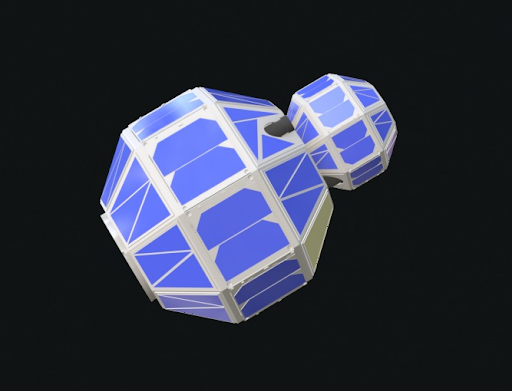
\includegraphics[width=0.75\textwidth]{Images/Figure 1.1.png}
    \caption[Conceptual visualization of the first operational stage of the LINKU tether mission]{Conceptual visualization of the first operational stage of the LINKU tether mission sequence between SAT-B and SAT-C. The figure depicts the initial pre-deployment configuration, in which SAT-C remains mechanically coupled to SAT-B prior to release. The subsequent mass separation initiates tether deployment, resulting in the progressive extension of the tether between the two masses. This stage represents the critical operational period for verifying nominal tether deployment and identifying potential anomalies through visual monitoring.}
    \label{fig:figure1.1}
\end{figure}

The primary role of the stereo vision system during deployment is to provide visual confirmation of the nominal extension sequence and support the identification of possible anomalies throughout the separation process. These anomalies may include:
\begin{itemize}
    \item Tether entanglement
    \item Asymmetric deployment
    \item Rebounds
    \item Unexpected oscillatory behavior
    \item Partial deployment
    \item Sudden changes in tether geometry
\end{itemize}

At this stage, maintaining continuous target centering within the image plane is inherently challenging due to spacecraft attitude variations immediately following separation. Because the cameras are rigidly mounted to the spacecraft structure, the apparent position of the tether and companion satellite may drift within the field of view during transient rotational motion.
\\\\
Additionally, maintaining fully stabilized attitude control throughout the deployment sequence may not be feasible due to constraints on spacecraft power, control authority, and volume. Consequently, the optical system must tolerate moderate angular deviations and transient motion while preserving sufficient situational awareness of the deployment region.
\\\\
For this reason, the optical configuration prioritizes wide-field observation capability during deployment operations, increasing the probability of maintaining partial or complete visibility of the tether and companion satellite despite residual spacecraft motion and pointing uncertainties.
\newpage
\clearpage

\noindent \textbf{Second operational stage: Post-deployment characterization}
\vspace{0.2cm}

After deployment stabilization, the tethered system transitions to a characterization stage focused on observing and analyzing tether dynamics under orbital conditions.

\begin{figure}[!ht]
    \centering
    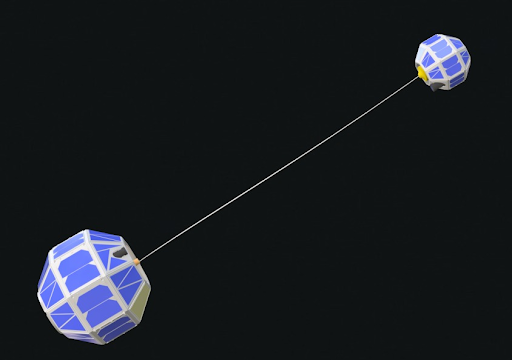
\includegraphics[width=0.75\textwidth]{Images/Figure 1.2.png}
    \caption[Conceptual visualization of the second operational stage of the LINKU tether mission]{Conceptual visualization of the second operational stage of the LINKU tether mission sequence between SAT-B and SAT-C. The figure illustrates the post-deployment configuration, where the tethered system reaches its nominal geometry and tends to align with the local radial (Nadir--Zenith) direction under gravity-gradient effects. This stage enables the characterization of tether geometry, dynamic behavior, and structural stability through visual observation and reconstruction techniques.}
    \label{fig:figure1.2}
\end{figure}

During this operational stage, the tethered system is expected to progressively evolve toward a gravity-gradient stabilized configuration, as shown in Figure \ref{fig:figure1.2}. Under this regime, the tether axis and the connected satellite masses tend to align approximately along the local radial direction of the orbit, with the system oscillating around the Nadir-Zenith axis that points toward and away from the Earth's center. However, residual oscillations, perturbations, and out-of-plane motion may still occur due to orbital disturbances and deployment transients.

The observational priorities during this stage include:

\begin{itemize}
    \item Characterization of tether curvature and spatial orientation
    \item Analysis of oscillatory motion
    \item Estimation of deformation behavior
    \item Generation of geometric datasets for dynamic model validation
\end{itemize}

Unlike the deployment stage, this operational regime prioritizes geometric reconstruction accuracy over wide-angle situational awareness. Consequently, image processing focuses on extracting the tether geometry from stereo imagery under highly constrained visual conditions.

In addition to tether observation, the stereo vision system architecture also enables exploratory evaluation of secondary proximity-awareness capabilities. In particular, the mission considers the possibility of reconstructing the relative geometry of the companion SAT-C mass from SAT-B stereo observations, providing preliminary information that may support future rendezvous or proximity-operation concepts without interfering with the primary tether-observation objectives.

\section{Instrument justification and data contextualization}

The stereo vision system is integrated into the LINKU mission to provide direct geometric observation of the tethered configuration and to contextualize measurements obtained from other onboard instruments. Conventional telemetry measurements provide only partial information regarding tether behavior. For example:

\begin{itemize}
    \item GNSS measurements provide relative separation vectors between spacecraft but do not describe the physical shape of the tether between them.
   \item Tether-tension measurements provide scalar force information at attachment points but cannot directly determine whether the tether remains straight, curved, oscillating, or partially entangled.
   \item Inertial measurements provide spacecraft attitude and rotational dynamics but do not directly capture the spatial geometry of the tether itself.
\end{itemize}

The stereo vision system complements these measurements by providing visual geometric information regarding the actual tether configuration throughout the mission.
\\\\
The resulting data has two principal operational functions:

\vspace{0.5cm}
\noindent \textbf{Qualitative operational awareness}
\vspace{0.2cm}

The visual observations provide direct situational awareness during deployment and post-deployment operations, enabling mission operators to identify anomalies or unexpected tether behavior through image inspection and geometric interpretation.

\vspace{0.5cm}
\noindent \textbf{Quantitative geometric reconstruction}
\vspace{0.2cm}

Stereo image processing enables the extraction of geometric information from the observed tether, including:
\begin{itemize}
    \item Three-dimensional spatial coordinates
    \item Curvature estimation
    \item Oscillation characterization
    \item Relative geometric evolution over time
\end{itemize}

These datasets are intended to support the validation of tether dynamic models and to complement the interpretation of GNSS, inertial, and tether-tension measurements obtained during flight operations.









%\paragraph{Phase 2: Post-Deployment Operations.} 
%Once deployed, the process becomes more predictable and the system transitions to a characterization mode. The tether is expected to align with the local vertical due to gravity-gradient stabilization, but it remains subject to orbital perturbations. Observational priorities include:
%\begin{itemize}
%    \item \textbf{Geometry Characterization:} Measuring 3D curvature and orientation relative to the orbital frame.
%    \item \textbf{Proximity Operations Support:} 3D reconstruction via space photogrammetry to determine the range and dimensions of SAT-C from the perspective of SAT-B, establishing foundational data for future rendezvous or approach applications.
%    \item \textbf{Model Validation:} Providing visual data to validate numerical simulations of tether dynamics.
%\end{itemize}

%\section{Environmental Constraints and Optical Scenarios}

%Effective imaging is strictly governed by the orbital environment. The following conditions define the operational scenarios for the camera system:

%\textbf{Illumination Cycles and Acquisition Triggers:} 
%Acquisition is restricted to the sunlit portion of the orbit. During eclipse periods, the lack of ambient light renders the tether invisible. To optimize power and storage, the satellite will not capture images blindly; it will determine favorable illumination scenarios by utilizing onboard orbital ephemeris data (propagators) and sun sensors to trigger the camera system only when lighting conditions are met.

%\begin{figure}[!ht]
%    \centering
%    \begin{minipage}{0.48\textwidth}
%        \centering
%        \includegraphics[width=\textwidth]{Images/imagen_izquierda.png}
%    \end{minipage}
%    \hfill
%    \begin{minipage}{0.48\textwidth}
%        \centering
%        \includegraphics[width=\textwidth]{Images/imagen_derecha.png}
%    \end{minipage}
%    \caption{Author-generated simulation of the tethered system under orbital illumination in Blender. Left: global view of the illumination geometry. Right: camera-perspective view used to evaluate the expected visual appearance of the tether.}
%    \label{fig:orbital_illumination}
%\end{figure}

%\textbf{Contrast, Saturation, and Resolution Limits:} 
%At an observation distance of approximately 100~m, the few-millimeter tether diameter subtends only 1--3 pixels on the sensor, placing the problem near the sub-pixel regime.

%Under high-contrast illumination, localized saturation may occur in the bright pixels associated with the tether response. In CMOS image sensors, \textbf{blooming} is caused by the spreading of excess photo-generated charge from over-saturated pixels into adjacent pixels, and one of its expected image artifacts is an increase in the size of saturated regions \cite{chao2013blooming,ailuri2016blooming}. 

%For the present mission concept, this effect is treated as a potential aid for \emph{initial detectability}, since saturation-induced spreading can enlarge the apparent footprint of an otherwise extremely thin feature. However, the apparent width under saturation does not represent the true physical diameter of the tether and should not be used directly for metrology; therefore, accurate geometry recovery must rely on specialized reconstruction methods rather than on the raw width of saturated imagery \cite{ailuri2016blooming}.


%\begin{figure}[!ht] % Cambiado a !ht
%    \centering
%    \includegraphics[width=0.8\textwidth]{Images/sim_contrast.png}
%    \caption{Author-generated conceptual illustration of the expected imaging response of a thin tether under high-contrast illumination in LEO. (a) Physical geometry. (b) Ideal sub-pixel sensor projection. (c) Local pixel saturation of the tether response. (d) Saturation-induced apparent footprint enlargement due to blooming. This figure is not reproduced from a prior publication; it was prepared by the author as a schematic interpretation supported by the sensor blooming mechanisms described in \cite{chao2013blooming,ailuri2016blooming}.}
%    \label{fig:tether_saturation}
%\end{figure}
